\chapter{Theory}

% maybe talk something about the breadcrumbs that lead me to where I am now?

This chapter provides an introduction to different tools that were used in the thesis to reach the stated aim. First we explain \textit{Formal Verification}, following it up with \textit{Model Checking} and its' strengths and weaknesses. Also some introduction to the model checking tool \textit{SPIN}, Simple Promela INterpreter, and its' input language \textit{Promela}. 

% approach ->
% As a starting point, I will consider a WSN where data is collected by sensors and then centrally processed by a server. Here the decision would be processed by the central unit and then propagated back to the sensors. Once the features of the decision procedure is characterized in this simple setting, I will then look at introducing more distributed computation capabilities in the network - e.g. by adding aggregators to manage a set of sensors or equipping all sensors with a computation unit to allow each of them to make decisions. To this aim, a computation unit would need to know what should be computed, how it should be computed and what has already been computed. This will allow the unit to decide if further collection is needed. 

% unit testing vs formal verification
%To analyze the system we wanted to improve, the project investigated different ways to design and verify a \wsn . For verifying, the two most relevant options were formal verification and testing (e.g. unit-testing) \todo{talk more about testing?}. Unit-testing is the technique of \ldots

%Formal verification on the other hand means that you, by logic, prove certain properties of the system and by so making sure the system works as intended. % really?

\section{Formal Verification}

The act of formal verification means to make use of mathematical techniques to make sure that a design upholds a defined functional correctness \cite{bjesse2005formal}.
This means, that if we assume we have the following: a model of a design, a description of the environment where the design is supposed to operate in and some properties we wish the design to uphold. With this information, one may want to construct some input sequences, that are in the allowed in domain of the environment, that would violate the properties stated. A common practice for finding such patterns today are random simulations or directed tests.
Formal verification allows for an extended approach to this, as it allows both to search for input sequences that violates the properties but also allows to mathematically prove that the stated properties holds when no input sequences exist.

\section{Model Checking}

A traditional approach to verifying concurrent systems is based on using extensive testing and simulation to find and eliminate unwanted occurrences from the system, but this way can easily miss crucial errors when the system that's being tested has a large number of possible states\cite{clarke1999model}. An alternative technique that was developed in the 1980's by Clarke et al. is called \textit{temporal logic model checking} or "Model Checking".

Model Checking is an automated technique to verify finite state concurrent systems, by letting a tool verify that a model holds for certain properties. The process of applying Model Checking to a design is separated into several tasks; \textit{modeling}, \textit{specification} and \textit{verification}. \\

\begin{itemize}
	\item[] \textbf{Modeling:} First task is to translate a design into a format which is accepted by a model checking tool. This is either a compilation task or a task in abstracting certain aspects of the design to eliminate irrelevant or unimportant details, due to limitations on time an memory. \\
	\item[] \textbf{Specification:} Second task is to state which properties the design is supposed to have. This is usually done using in a logical formalism, commonly in temporal logic, which can express assertions on a system evolving over time. \\
	\item[] \textbf{Verification:} The final step is allowing the tool to verify the specification on the model. This will either be a positive result, meaning the model satisfies the properties, or a negative result where the properties aren't. A negative result can also be that the model's state space is too large to fit into a computer, which will require the model to be further abstracted to be verified.
\end{itemize}


\subsection{Model Checking Workflow}

%\textit{show a structure of a model checking workflow}\todo{show structure of model checking workflow}

The use of model checking in practice typically follows the workflow in Figure~\ref{fig:mc_workflow}. A design is translated into a description, that the model checker can read, and a specification of wanted or unwanted behavior is translated into a property. Then the model checker will produce a result which is either that the property is upheld or an error explaining how the property is invalidated\cite{clarke1999model}. 

\begin{figure}[ht]
    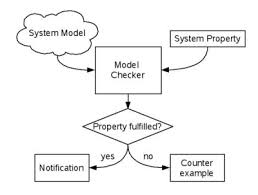
\includegraphics[resolution=100]{include/figures/mc_workflow}
    \caption{Workflow of Model Checking}
    \label{fig:mc_workflow}
\end{figure}

\section{SPIN}

The model checking tool used in this thesis is called SPIN, an abbreviation of Simple Promela Interpreter. The SPIN tool allows to create an abstract model of a system, specifying properties that the model must hold and then verify them to see if there is possible system state that invalidates it. SPIN verification models are focused on proving the correctness of process interactions.\cite{holzmann1997model} Process interactions can be specified in several ways using SPIN; rendevouz primitives, asynchronous message passing, shared variables or a combination of these. 

% discuss difference from SPIN to other tools?

% discuss how you can use SPIN to find errors

\subsection{Promela}
Promela is a specification language with its' focus on modeling process synchronization and coordination rather than computation. Therefore the language targets the description of conurrent software systems, rather than the description of hardware circuits, which is more common for other model checking applications\cite{holzmann1997model}.
The features in the Promela language allows for description of concurrent processes and communication through message passing over buffered or rendevouz(unbuffered) channels. \\

% discuss the simplicity of promela for reaching better abstraction

\textbf{Promela Example} \\

To give an impression of Promela's syntax, Listing~\ref{lst:example} serves as an small example that captures most of the concepts used in this thesis. The example models an procedure called \textit{environment}, receiving a message \texttt{meter} on the channel \texttt{envChan}. Then the process undeterministically choses one of the two responses in the guard statement and responds back on the same channel. Worth noting is that most part of the model is captured in an \texttt{atomic}-statement, this means that when the request is received, this process will be allowed to execute the rest of the \texttt{atomic}-statement without any interleaving. 
Since this process flow isn't realistic in a concurrent system, where interleaving is prone to occur, all usage of \texttt{atomic} has to be explained and carefully motivated. 

\begin{lstlisting}[caption={Promela Example},label={lst:example},language=Promela, numbers=left, basicstyle=\footnotesize, tabsize=2]
active proctype Environment() {

Idle:  
	if
	:: atomic { 
		envChan ? meter ->  
			if
			:: envChan ! bigData;
			:: envChan ! smallData;
			fi; 
			goto Idle;
	}
	fi;
}
\end{lstlisting}

\subsection{Properties in SPIN}

% intro linear time logic?

% something explanatory?

\textbf{Specification} \\

In order to prove or disprove a property using SPIN, we must first state them in some formal notation\ref{spinreferencemanualbook}. This can be done by either using \texttt{assertion}-statements, to ensure a property at a certain point in time, or using LTL to prove properties over an entire system trace. 
Except the operators inherited from propositional logic (\textit{negation}, \textit{conjunction}, \textit{equivalence}, \textit{implication}, etc.) LTL also provides the temporal operators such as \textit{always}, \textit{eventually} and \textit{until}. 

\begin{itemize}
	\setlength\itemsep{1em}
	\item[] \textbf{Always} ($\Box$) states that a property has to hold on the entire subsequent path, e.g $\Box a$ means that the condition $a$ always holds true. In promela this is either written as \texttt{always} or \texttt{[]}.
	\item[] \textbf{Eventually} ($\Diamond$) states that a property has to hold somewhere on the subsequent path, meaning that $\Diamond a$ means that $a$ must hold in the current state or in some future state. This is written in promela as \texttt{<>} or \texttt{eventually}.
	\item[] \textbf{Until} ($U$) captures a relative behavior between two condditions, e.g. $a \text{ U } b$ means that $a$ must hold true atleast until $b$ holds true. In promela this is written as \texttt{U} or \texttt{until}.
 \end{itemize}

For a complete description of Linear Time Logic and its' semantics in SPIN, see Holzmann (2003, p. 135-139). \\

\textbf{Verification} \\

Spin allows us to either prove properties that always should hold true (safety properties) or error behaviors (i.e. properties that should never hold). When verifying safety properties in Spin, instead of trying to prove that a property holds true in each possible system state, it tries to find a state in which the property is invalidated. This is intuitively a faster way of finding erroneous behavior since when the verification finds one counterexample to the stated property, it no longer needs to search other states. 
So when running the verification, Spin negates the specified property and then attempts to find a system trace in which the negated property holds. If this is successful, then the property can be violated. Otherwise, if no such trace exists, the property is verified to always hold true.

\subsection{Problem space reduction}

% mention abstraction and reducing the model 

There are two strategies that SPIN uses to reduce the number of states generated in verification \ref{spinreferencemanualbook}. The aims of them are; "to reduce the amount of reachable system states that must be searched to verify properties, or to reduce the amount of memory that is needed to store each state".

One strategy to achieve this is called partial order reduction, which relies on selecting and examining only a subset of all possible execution paths. An example of this is by detecting interleaving of processes which relative ordering do not affect the final outcome of the execution, with regards to the property being verified. 

%\todo{mention clarke et al?}

Another strategy SPIN uses is stutter equivalence. As explained by Peled, Wilke \& Wolper in 1995\cite{peled1996algorithmic}: “a pair of sequences are considered to be equivalent if they differ in at most the number of times a state may adjacently repeat”. Spin's partial order reduction strategy assumes this, and by so only guarantees verification for stutter invariant properties. This makes it impossible to verify properties containing the \textit{next}-operator\ref{spinreferencemanualbook}, meaning an LTL formula which doesn't use the \textit{next}-operator is by guarantee also stutter invariant.

%\section{Other stuff} % this section has been moved from §4


%This definition, though focusing on a different target system, still held some context to our work and was used a reference point for the initial work on over-collection.

%mention that their targets were primary smartphones demanding too much information?

%begin differently
%Yibin Li et al defined over-collection, or "data over-collection", as . % describe their motivation behind this and perhaps some conclusion they came to.

% says who?

% mention others definitions' of over-collection



%Over-Collection is the state or process which a system collects data beyond the scope of it's required parameters. 

% used
% As mentioned in the background, there are several examples of applications where personal data is collected from users \todo{link some of them here}. Each of these applications have different purposes for collecting data and different levels of privacy. \\ \textbf{Definition (informal):} If an entitity collects more data than required to complete it's purpose, it's over-collecting. \\ From this definition, for instance, if in the article from the Chicago Tribunal \todo{insert ref}, they mentioned that after the nodes had read and analyzed the data, the captured images would be destroyed. This is a step taken to prevent over-collection. If instead the image would be stored after the analysis had been completed, e.g. in a central server, this would be collecting more data than required and the system would be over-collecting. \\ This means that over-collection is a state of which a system can be in. For our models, we've modeled it as another state. In practice though, a system that collects data without some restriction, could easily be over-collecting always and never. By letting a system knowing more specifically what to look for and discard more of the gathered data, would make it "smarter" in an IoT-sense, and also to better prevent over-collection. \\ To formalize this, if we have system that collects data, and at some point in the system it's collected enough data - for what's required. At this state, if the system would collect data, without first "leaving" this state, the system would be over-collecting. 

% refer to the definitions by Pfitzmann




%A \wsn primary objective is to collect data from an observed source and let a processing unit analyze the state of it. 

%In the paper \textit{insert reference to chapter 2 here}, they defined \textit{Data Over-Collection} to be "Collecting data more than enough on original function while within the permission scope". 

%For this to be true, we make the assumption that it exists a state for the system where the process of collecting data isn't required for the system to function the way it's intended. This could arise from a number of origins, either that a threshold has been reached and the system is no longer stable or that 

%Consider a collection process collecting some personal data from a users. The process is only interested in collecting as much data as possible and storing it at a central server for future processing. We can assume that the process will need a good quantity of data entries to extract relevant information from the data. If we assume that the program doesn't remove any data it's collected, we can safely say that at some point the system will have collected enough data to accomplish the tasks it's designed to do and beyond that point it's collected more than it requires.

% describe what over-collection means
%With a collection-process 'mindlessly' collecting personal data and storing it, we can assume that there's state where the collection has collected more data than it requires to complete whatever function the system is designed to do. 

%\begin{definition}{def:Coll}{}
%(Collecting)

%A process $P$ collects a data point $d$

%A process $P$ collects a data point $d$ in a state $s$ if after leaving the state then $d \in \{P_{c'} \setminus P_{c}\}$.

%A process $P$ collects a data point $d$ in a state $s$ if after leaving state $s$ ($s_{+1}$) then $d \in P.lvars$\todo{promela syntax for local variables, should be something else}.
%\end{definition}

%\begin{definition}{def:ToFunc}{}
%(To Function)

%\textit{if a process P yields a valid result by a specific amount of input parameters, we say it requires these input parameters}
%\end{definition}

% shall i really include time as a variable in my definition? snapshots seems better.
% We can consider two possibilities of systems, one where the system doesn't remove data from it's collection on it's own and one where it removes data over time.

%\begin{definition}{def:OverColl}{} 
%(Over-Collection)

%\textit{if a process P collects more data than it "requires to function", we say a process is over-collecting.}
%\end{definition} 

%\textbf{Formal Definition: } 
%Let a process P be able to collect data entries and to evaluate boolean expressions. 

%$P_{collect}: D \cup P_{collection}$

%where $P_{collection}$ means the set of data entries $(D_1,D_2,\ldots)$ collected, intially $\emptyset$, and $D$ is a new data entry being collected.

%$P_{eval}: D \rightarrow \textbf{Bool}$

%Let a service $S(x, y, ...)$ be a boolean expression depending on variables $x, y, ...$ 

%We say the process $P$ dedicated to the service $S$, noted $<P,S>$, over-collects data if and only if $P$ collects any data concerning one of the variables appearing in $S$ after $S$ has been evaluated to be true.

%$<P,S>$ over-collects iff $ \{ D \in P_{collection} \} \wedge \{ P_{eval}(D) = \textbf{True}\}$ \todo{something like that, but with S}

%$P = (C,E)$ $C$ is a finite set where the elements are tuples of $c \in C : c = (x,y,...)$ called data entries. $E: c \in C \rightarrow \textbf{Bool}$ (E is a function on an element in C with a resulting boolean value.) if $\left\{ { E: \exists c \in C \rightarrow \textbf{True} } \right\} \wedge \left\{ { S(x,y,...) \rightarrow \textbf{True} } \right\}$ and $c = (x,y,...)$ (translation between variables and c).

%Let $\textbf{D}_C$ be a new data point not in the collection and $\textbf{D}$ be the current stored collection of data. Let $|D|$ be the amount of data entries in $\textbf{D}$ and $\textbf{F}$ be a fixed number describing the amount of data a process requires to function.  

%So consider a system that is not in a over-collective state ($|\textbf{D}| < \textbf{F}$) is receiving a new entry point to it's collection; 

%\[ \textbf{D} + \textbf{D}_C = \textbf{D}' \]

%Where '+' means the operation of appending the data to the collection. So then if:

%\[ |\textbf{D}'| \geq \textbf{F} \]

%Then a system is over-collecting.

% assume non-dissipating? personal data not being removed?

% formal formulation (like non-inference)

%*overcollection-examples*

%*define over-collection*



% how decisions are used

% what they are

% how they can be used

% ----------

%introduction leading up to what we need it for.

%To formulate the problem on whether or not to act on information, the thesis used an expression we called \textit{decisions}. We specified that for a system to decide whether or not it was over-collecting; "a decision had to be taken". 

%\textit{something about algorithms}

%\textit{what is a decision procedure?}

\subsection{Decision Procedures}

In our research of over-collection, the project realized we needed some algorithmic way for a system to determine if it was over-collecting or not. To this end, we studied \textit{decision problems}. A decision problem is a question expressed in some formal system that can be stated a "yes-no" question. And an algorithm used for solving decision problems is called a \textit{decision procedure}, which terminates with a "yes" or "no" answer\cite{decisionproceduresbook}. 

% decision procedure has a wide range of uses?
Decision procedures has a wide range of uses and is increasingly being used in hardware verification and theorem proving tools\cite{ganesh2007decision}. Some examples of such decision procedures are Yices, SVC, CVC Lite, UCLID \cite{dutertre2006fast, barrett1996validity, barrett2004cvc, lahiri2004uclid}. Besides theorem-proving and hardware verification, decision procedures are also increasingly being used in large-scale program analysis, bug finding and test generation tools (e.g. \cite{newsome2006replayer, cadar2008exe}).

%A formal system for expressing decision problems could for example be propositional logic, a simple example of its' syntax can be seen in Figure~\ref{fig:prop_logic}. 

% mention its FOL? 
%\begin{figure}[ht]
%	\[ x_1 \land (x_2 \lor \neg x_3) \]
%    \caption{A simple example of a propsitional logic}
%    \label{fig:prop_logic}
%\end{figure}





% mention 

% 

%In the book "Decision Procedures - An Algorithmic Point of View" by Kroening and Strichman





% mention difference from FOL and onwards?

%This means that there had to be an algorithm in place for the system to yield a "yes or no" answer when invoked. This is known as a \textit{decision procedure}\cite{decisionproceduresbook} 

%\textit{show example of a decision procedure}

%\textit{explain the point of it}

%From the Definition~\ref{def:OverColl} we understand it's not uncommon for processes to collect more data than they require. 

% A single sensor node usually\cite{WSN_a_survey} doesn't hold enough information about the system state to 


%\subsubsection{Formal Definition}

%\begin{definition}{}{}
%\label{def:DecProc}
%(Decision Process)

%A process is called a decision process for T if it is sound and complete with respect to every formula of T.
%\end{definition}

%\textit{Definition \ref{def:DecProc} also requires some more definitions, but this is an important one so added it for now.}

%\begin{definition}{}{}
%\label{def:DecComplete}
%(Completeness of a procedure)

%A procedure for the decision problem is complete if 
%\begin{itemize}
%\item it always terminates (termination), and
%\item it returns "Valid" when the input is valid. (soundness)
%\end{itemize}

%\end{definition}


%A decision \todo{rewrite} is a control message sent through the network forcing an action to be taken\todo{witness? semantics?}, in this report that's mainly when over-collection is occurring. This can for example mean that the server is telling one (or several) collection nodes that they should shut down or wait until sending again. If the nodes are also computing data they can still be kept doing so but without sending communication throughout the network until notified again. The source of the decision depends on if the network has a centralized processing unit (f.e. a master-slave relation) or if computations are decentralized and each processing unit makes decision on their own and uses communication to forward processed data to a storage server. 

%\textbf{Definition: } A message sent in the network is considered a decision if it changes the behavior of an actor.

%*formally define decisions* ?